% Generated by Sphinx.
\def\sphinxdocclass{report}
\documentclass[a4paper,12pt,spanish]{sphinxmanual}
\usepackage[utf8]{inputenc}
\DeclareUnicodeCharacter{00A0}{\nobreakspace}
\usepackage{cmap}
\usepackage[T1]{fontenc}
\usepackage{babel}
\usepackage{times}
\usepackage[Sonny]{fncychap}
\usepackage{longtable}
\usepackage{sphinx}
\usepackage{multirow}


\title{Programación de Móviles}
\date{26 de September de 2014}
\release{1.0}
\author{Oscar Gomez}
\newcommand{\sphinxlogo}{}
\renewcommand{\releasename}{Publicación}
\makeindex

\makeatletter
\def\PYG@reset{\let\PYG@it=\relax \let\PYG@bf=\relax%
    \let\PYG@ul=\relax \let\PYG@tc=\relax%
    \let\PYG@bc=\relax \let\PYG@ff=\relax}
\def\PYG@tok#1{\csname PYG@tok@#1\endcsname}
\def\PYG@toks#1+{\ifx\relax#1\empty\else%
    \PYG@tok{#1}\expandafter\PYG@toks\fi}
\def\PYG@do#1{\PYG@bc{\PYG@tc{\PYG@ul{%
    \PYG@it{\PYG@bf{\PYG@ff{#1}}}}}}}
\def\PYG#1#2{\PYG@reset\PYG@toks#1+\relax+\PYG@do{#2}}

\expandafter\def\csname PYG@tok@vg\endcsname{\def\PYG@tc##1{\textcolor[rgb]{0.73,0.38,0.84}{##1}}}
\expandafter\def\csname PYG@tok@sc\endcsname{\def\PYG@tc##1{\textcolor[rgb]{0.25,0.44,0.63}{##1}}}
\expandafter\def\csname PYG@tok@nv\endcsname{\def\PYG@tc##1{\textcolor[rgb]{0.73,0.38,0.84}{##1}}}
\expandafter\def\csname PYG@tok@vc\endcsname{\def\PYG@tc##1{\textcolor[rgb]{0.73,0.38,0.84}{##1}}}
\expandafter\def\csname PYG@tok@nd\endcsname{\let\PYG@bf=\textbf\def\PYG@tc##1{\textcolor[rgb]{0.33,0.33,0.33}{##1}}}
\expandafter\def\csname PYG@tok@s2\endcsname{\def\PYG@tc##1{\textcolor[rgb]{0.25,0.44,0.63}{##1}}}
\expandafter\def\csname PYG@tok@kr\endcsname{\let\PYG@bf=\textbf\def\PYG@tc##1{\textcolor[rgb]{0.00,0.44,0.13}{##1}}}
\expandafter\def\csname PYG@tok@gu\endcsname{\let\PYG@bf=\textbf\def\PYG@tc##1{\textcolor[rgb]{0.50,0.00,0.50}{##1}}}
\expandafter\def\csname PYG@tok@nc\endcsname{\let\PYG@bf=\textbf\def\PYG@tc##1{\textcolor[rgb]{0.05,0.52,0.71}{##1}}}
\expandafter\def\csname PYG@tok@nn\endcsname{\let\PYG@bf=\textbf\def\PYG@tc##1{\textcolor[rgb]{0.05,0.52,0.71}{##1}}}
\expandafter\def\csname PYG@tok@m\endcsname{\def\PYG@tc##1{\textcolor[rgb]{0.13,0.50,0.31}{##1}}}
\expandafter\def\csname PYG@tok@gi\endcsname{\def\PYG@tc##1{\textcolor[rgb]{0.00,0.63,0.00}{##1}}}
\expandafter\def\csname PYG@tok@vi\endcsname{\def\PYG@tc##1{\textcolor[rgb]{0.73,0.38,0.84}{##1}}}
\expandafter\def\csname PYG@tok@err\endcsname{\def\PYG@bc##1{\setlength{\fboxsep}{0pt}\fcolorbox[rgb]{1.00,0.00,0.00}{1,1,1}{\strut ##1}}}
\expandafter\def\csname PYG@tok@nb\endcsname{\def\PYG@tc##1{\textcolor[rgb]{0.00,0.44,0.13}{##1}}}
\expandafter\def\csname PYG@tok@c\endcsname{\let\PYG@it=\textit\def\PYG@tc##1{\textcolor[rgb]{0.25,0.50,0.56}{##1}}}
\expandafter\def\csname PYG@tok@go\endcsname{\def\PYG@tc##1{\textcolor[rgb]{0.20,0.20,0.20}{##1}}}
\expandafter\def\csname PYG@tok@s1\endcsname{\def\PYG@tc##1{\textcolor[rgb]{0.25,0.44,0.63}{##1}}}
\expandafter\def\csname PYG@tok@w\endcsname{\def\PYG@tc##1{\textcolor[rgb]{0.73,0.73,0.73}{##1}}}
\expandafter\def\csname PYG@tok@kp\endcsname{\def\PYG@tc##1{\textcolor[rgb]{0.00,0.44,0.13}{##1}}}
\expandafter\def\csname PYG@tok@kt\endcsname{\def\PYG@tc##1{\textcolor[rgb]{0.56,0.13,0.00}{##1}}}
\expandafter\def\csname PYG@tok@gr\endcsname{\def\PYG@tc##1{\textcolor[rgb]{1.00,0.00,0.00}{##1}}}
\expandafter\def\csname PYG@tok@na\endcsname{\def\PYG@tc##1{\textcolor[rgb]{0.25,0.44,0.63}{##1}}}
\expandafter\def\csname PYG@tok@cm\endcsname{\let\PYG@it=\textit\def\PYG@tc##1{\textcolor[rgb]{0.25,0.50,0.56}{##1}}}
\expandafter\def\csname PYG@tok@nl\endcsname{\let\PYG@bf=\textbf\def\PYG@tc##1{\textcolor[rgb]{0.00,0.13,0.44}{##1}}}
\expandafter\def\csname PYG@tok@kc\endcsname{\let\PYG@bf=\textbf\def\PYG@tc##1{\textcolor[rgb]{0.00,0.44,0.13}{##1}}}
\expandafter\def\csname PYG@tok@mi\endcsname{\def\PYG@tc##1{\textcolor[rgb]{0.13,0.50,0.31}{##1}}}
\expandafter\def\csname PYG@tok@ne\endcsname{\def\PYG@tc##1{\textcolor[rgb]{0.00,0.44,0.13}{##1}}}
\expandafter\def\csname PYG@tok@s\endcsname{\def\PYG@tc##1{\textcolor[rgb]{0.25,0.44,0.63}{##1}}}
\expandafter\def\csname PYG@tok@nf\endcsname{\def\PYG@tc##1{\textcolor[rgb]{0.02,0.16,0.49}{##1}}}
\expandafter\def\csname PYG@tok@bp\endcsname{\def\PYG@tc##1{\textcolor[rgb]{0.00,0.44,0.13}{##1}}}
\expandafter\def\csname PYG@tok@mo\endcsname{\def\PYG@tc##1{\textcolor[rgb]{0.13,0.50,0.31}{##1}}}
\expandafter\def\csname PYG@tok@sb\endcsname{\def\PYG@tc##1{\textcolor[rgb]{0.25,0.44,0.63}{##1}}}
\expandafter\def\csname PYG@tok@se\endcsname{\let\PYG@bf=\textbf\def\PYG@tc##1{\textcolor[rgb]{0.25,0.44,0.63}{##1}}}
\expandafter\def\csname PYG@tok@gs\endcsname{\let\PYG@bf=\textbf}
\expandafter\def\csname PYG@tok@gt\endcsname{\def\PYG@tc##1{\textcolor[rgb]{0.00,0.27,0.87}{##1}}}
\expandafter\def\csname PYG@tok@sh\endcsname{\def\PYG@tc##1{\textcolor[rgb]{0.25,0.44,0.63}{##1}}}
\expandafter\def\csname PYG@tok@gp\endcsname{\let\PYG@bf=\textbf\def\PYG@tc##1{\textcolor[rgb]{0.78,0.36,0.04}{##1}}}
\expandafter\def\csname PYG@tok@c1\endcsname{\let\PYG@it=\textit\def\PYG@tc##1{\textcolor[rgb]{0.25,0.50,0.56}{##1}}}
\expandafter\def\csname PYG@tok@ge\endcsname{\let\PYG@it=\textit}
\expandafter\def\csname PYG@tok@gh\endcsname{\let\PYG@bf=\textbf\def\PYG@tc##1{\textcolor[rgb]{0.00,0.00,0.50}{##1}}}
\expandafter\def\csname PYG@tok@sx\endcsname{\def\PYG@tc##1{\textcolor[rgb]{0.78,0.36,0.04}{##1}}}
\expandafter\def\csname PYG@tok@il\endcsname{\def\PYG@tc##1{\textcolor[rgb]{0.13,0.50,0.31}{##1}}}
\expandafter\def\csname PYG@tok@kn\endcsname{\let\PYG@bf=\textbf\def\PYG@tc##1{\textcolor[rgb]{0.00,0.44,0.13}{##1}}}
\expandafter\def\csname PYG@tok@o\endcsname{\def\PYG@tc##1{\textcolor[rgb]{0.40,0.40,0.40}{##1}}}
\expandafter\def\csname PYG@tok@si\endcsname{\let\PYG@it=\textit\def\PYG@tc##1{\textcolor[rgb]{0.44,0.63,0.82}{##1}}}
\expandafter\def\csname PYG@tok@mf\endcsname{\def\PYG@tc##1{\textcolor[rgb]{0.13,0.50,0.31}{##1}}}
\expandafter\def\csname PYG@tok@ow\endcsname{\let\PYG@bf=\textbf\def\PYG@tc##1{\textcolor[rgb]{0.00,0.44,0.13}{##1}}}
\expandafter\def\csname PYG@tok@gd\endcsname{\def\PYG@tc##1{\textcolor[rgb]{0.63,0.00,0.00}{##1}}}
\expandafter\def\csname PYG@tok@kd\endcsname{\let\PYG@bf=\textbf\def\PYG@tc##1{\textcolor[rgb]{0.00,0.44,0.13}{##1}}}
\expandafter\def\csname PYG@tok@sd\endcsname{\let\PYG@it=\textit\def\PYG@tc##1{\textcolor[rgb]{0.25,0.44,0.63}{##1}}}
\expandafter\def\csname PYG@tok@ss\endcsname{\def\PYG@tc##1{\textcolor[rgb]{0.32,0.47,0.09}{##1}}}
\expandafter\def\csname PYG@tok@cp\endcsname{\def\PYG@tc##1{\textcolor[rgb]{0.00,0.44,0.13}{##1}}}
\expandafter\def\csname PYG@tok@nt\endcsname{\let\PYG@bf=\textbf\def\PYG@tc##1{\textcolor[rgb]{0.02,0.16,0.45}{##1}}}
\expandafter\def\csname PYG@tok@k\endcsname{\let\PYG@bf=\textbf\def\PYG@tc##1{\textcolor[rgb]{0.00,0.44,0.13}{##1}}}
\expandafter\def\csname PYG@tok@no\endcsname{\def\PYG@tc##1{\textcolor[rgb]{0.38,0.68,0.84}{##1}}}
\expandafter\def\csname PYG@tok@cs\endcsname{\def\PYG@tc##1{\textcolor[rgb]{0.25,0.50,0.56}{##1}}\def\PYG@bc##1{\setlength{\fboxsep}{0pt}\colorbox[rgb]{1.00,0.94,0.94}{\strut ##1}}}
\expandafter\def\csname PYG@tok@sr\endcsname{\def\PYG@tc##1{\textcolor[rgb]{0.14,0.33,0.53}{##1}}}
\expandafter\def\csname PYG@tok@mh\endcsname{\def\PYG@tc##1{\textcolor[rgb]{0.13,0.50,0.31}{##1}}}
\expandafter\def\csname PYG@tok@ni\endcsname{\let\PYG@bf=\textbf\def\PYG@tc##1{\textcolor[rgb]{0.84,0.33,0.22}{##1}}}

\def\PYGZbs{\char`\\}
\def\PYGZus{\char`\_}
\def\PYGZob{\char`\{}
\def\PYGZcb{\char`\}}
\def\PYGZca{\char`\^}
\def\PYGZam{\char`\&}
\def\PYGZlt{\char`\<}
\def\PYGZgt{\char`\>}
\def\PYGZsh{\char`\#}
\def\PYGZpc{\char`\%}
\def\PYGZdl{\char`\$}
\def\PYGZhy{\char`\-}
\def\PYGZsq{\char`\'}
\def\PYGZdq{\char`\"}
\def\PYGZti{\char`\~}
% for compatibility with earlier versions
\def\PYGZat{@}
\def\PYGZlb{[}
\def\PYGZrb{]}
\makeatother

\renewcommand\PYGZsq{\textquotesingle}

\begin{document}
\shorthandoff{"}
\maketitle
\tableofcontents
\phantomsection\label{index::doc}


Índice:


\chapter{Análisis de tecnologías para aplicaciones en dispositivos móviles:}
\label{index:analisis-de-tecnologias-para-aplicaciones-en-dispositivos-moviles}\label{index:prog-multimedia-y-de-dispositivos-moviles}

\section{Puntos iniciales}
\label{index:puntos-iniciales}\begin{itemize}
\item {} 
En primer lugar, en \href{http://10.8.0.253}{http://10.8.0.253} se puede encontrar un servidor.

\item {} 
Los apuntes también se podrán encontrar a diario en \href{http://oscarmaestre.github.io}{http://oscarmaestre.github.io}

\item {} 
Existen fotocopias con la programación, criterios, etc... en la mesa del profesor. En cualquier caso, están colgadas en la página del centro \href{http://www.iesmaestredecalatrava.es}{http://www.iesmaestredecalatrava.es} (buscar el apartado ``Presentaciones''

\item {} 
Si se desea acceder a algún fichero individual de los apuntes puede hacerse en las página siguiente
\begin{itemize}
\item {} 
\href{https://github.com/OscarMaestre/Moviles}{https://github.com/OscarMaestre/Moviles}

\item {} 
\href{https://github.com/OscarMaestre/ServiciosYProcesos}{https://github.com/OscarMaestre/ServiciosYProcesos}

\end{itemize}

\end{itemize}


\section{Sistemas operativos para dispositivos móviles. Características.}
\label{index:sistemas-operativos-para-dispositivos-moviles-caracteristicas}
El desarrollo para la telefonía móvil es un campo que se encuentra en plena expansión. El número de teléfonos no deja de crecer y las necesidades de programación de los mismos tampoco. En ese sentido existen diversas plataformas de desarrollo a tener en cuenta al empezar a programar.
\begin{itemize}
\item {} 
Android: es el más numeroso de lejos. La mayor parte del mercado usa esta plataforma. El hecho de que Google ofrezca \emph{completamente gratis} el sistema operativo para los fabricantes y el entorno para los programadores lo ha hecho crecer hasta desbancar a su competidor. Google solo se ocupa de la venta de apps y ese es su nicho de beneficios.

\item {} 
iOS: Utiliza una filosofía completamente distinta que es controlar todo el proceso desde el desarrollo hasta la distribución de aplicaciones. Ese control se hace por medio del pago de licencias y de la unicidad de la distribución.

\item {} 
Windows Phone: es el sistema de Microsoft que ha lanzado más o menos recientemente y que aún está por ver si consigue una cuota de mercado significativa o no.

\item {} 
FirefoxOS: se centra principalmente en mercados emergentes (con el objetivo a largo plazo de ganar cuota de mercado) su filosofía es la misma del software libre.

\item {} 
Bada: Es la plataforma de Samsung creada exclusivamente para sus teléfonos. Es muy poco usada fuera de Corea del Sur.

\item {} 
Symbian: surge de un antiguo sistema creado para las PDA, está prácticamente descatalogado en el desarrollo para telefonía móvil.

\item {} 
Tizen: una plataforma relativamente nueva. Al igual que Android es gratis y además tiene el respaldo de Intel.

\item {} 
Jolla: surge en los países nórdicos con una filosofía similar al software libre pero con la salvedad de que, de momento, solo se ejecuta en sus teléfonos (que son de gama alta)

\end{itemize}

En cuanto a la tecnología hay diferencias sustanciales entre ellas:
\begin{itemize}
\item {} 
Android: pensado principalmente para ser programado en Java (aunque se puede llegar a usar C++ con un kit aparte).

\item {} 
iOS: usa Objective-C que lo separa mucho del resto de plataformas. El entorno exige el pago de una licencia, el SO exige una licencia y el poner aplicaciones a la venta exige otra.

\item {} 
Windows Phone: usa Visual Studio que es una herramienta muy potente y usa la plataforma .NET.

\item {} 
FirefoxOS: usa HTML y Javascript.

\item {} 
Symbian y otros también permiten el uso de HTML y JS.

\item {} 
Tizen permite dos opciones: C++ o HTML/JS

\item {} 
Jolla/Sailfish: usa C++.

\item {} 
Bada usa C++.

\end{itemize}

En este curso se usara Android con Java como lenguaje de desarrollo.


\section{Limitaciones}
\label{index:limitaciones}
Programar un teléfono móvil implica preparar nuestro programa para situaciones que no son de importancia en los ordenadores de escritorio o que incluso no existen.
\begin{itemize}
\item {} 
Desconexión: un teléfono puede perder el fluido eléctrico sin aviso o perder la conexión de red de forma repentina.

\item {} 
Seguridad: un teléfono puede ser accesible desde cualquier punto del planeta lo que puede poner en grave riesgo la privacidad del usuario.

\item {} 
Memoria: la cantidad de memoria de estos dispositivos es mucho más reducida que los equipos de escritorio.

\item {} 
Consumo batería: la cantidad de código que se ejecuta implica disminuir la cantidad de batería del usuario.

\item {} 
Almacenamiento: la cantidad de espacio para almacenar ficheros en estos dispositivos es muy variable y a veces prácticamente inexistente.

\end{itemize}


\section{Entornos integrados de trabajo.}
\label{index:entornos-integrados-de-trabajo}
En este apartado vamos a hablar de los distintos entornos que se pueden usar para programar teléfonos móviles.
\begin{itemize}
\item {} 
Eclipse.

\item {} 
XCode para iOS.

\item {} 
Android Studio.

\item {} 
NetBeans.

\item {} 
Visual Studio (para Windows Phone).

\item {} 
¿Visual Kaffe?

\item {} 
Línea de comandos.

\item {} 
Appcelerator.

\end{itemize}


\section{Android Studio}
\label{index:android-studio}
Android Studio es el entorno oficial de programación de Google. Como tal, es probablemente la herramienta del futuro si bien tiene diversas desventajas.
\begin{itemize}
\item {} 
Aún está en fase beta y según los documentos de instalación aún puede cambiar mucho sin previo aviso.

\item {} 
Requiere una máquina más potente que los otros: de no ser así el proceso de edición-compilación-ejecución se vuelve demasiado lento.

\end{itemize}


\section{Eclipse}
\label{index:eclipse}
Eclipse ha sido desde los comienzos la herramienta ofrecida por Google para programar en Android. De hecho, en su página se ofrece el ``Android Developer Tools Bundle'' que contiene absolutamente todo lo necesario para trabajar.

En este manual será la herramienta que se utilizará para los ejemplos.


\section{La línea de comandos}
\label{index:la-linea-de-comandos}
La línea de comandos es el entorno más ligero. Además ofrece grandes ventajas en cuanto a la automatización de tareas, y de hecho Google ofrece el kit de desarrollo adaptado a la línea de comandos. El inconveniente principal es que algunos desarrolladores no están muy acostumbrados a ella.


\section{El primer proyecto}
\label{index:el-primer-proyecto}
Cuando se instala el Android Developer Bundle y se arranca Eclipse podremos utilizar un pequeño asistente para crear la primera aplicación. Para ello, en el menú \code{File-New} elegiremos la opción \code{Android Application Project}, mostrándonos una ventana que debería ser parecida a la siguiente figura.
\begin{figure}[htbp]
\centering
\capstart

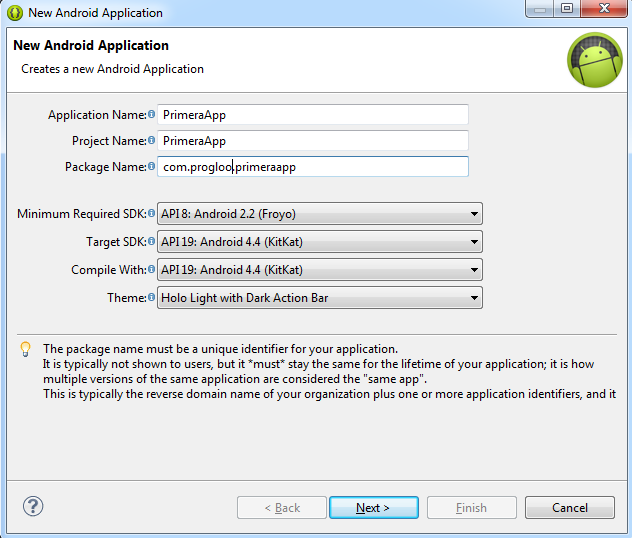
\includegraphics{asistente1.png}
\caption{Datos iniciales de la aplicación Android}\end{figure}

En ella deberemos prestar atención a los siguientes elementos:
\begin{itemize}
\item {} 
\emph{Minimum required SDK} : es la versión de Android mínima que necesitará en su móvil/tablet quien desee instalar la aplicación. Si se tiene la tentación de poner la versión 1.0 se debe tener en cuenta que también se dispondrán de menos clases y métodos para construir la app. La versión 8 (Android 2.1) es un valor razonable a día de hoy.

\item {} 
\emph{Target SDK} : es la versión de Android para la cual hemos optimizado la aplicación. En todo este manual se usará la versión 19 de Android (o Android 4.4)

\item {} 
\emph{Compile with} : Android tiene varias versiones y podemos utilizar una versión posterior para optimizar una aplicación orientada a un Android más antiguo. Sin embargo, normalmente no lo haremos y usaremos la misma versión que en el Target SDK, es decir, la 19.

\item {} 
\emph{Theme} : las aplicaciones pueden tener diversos temas o ``skins''. Google ofrece algunos estilos predeterminados, pero no haremos especial hincapie en el diseño, solo en la programación. Usaremos el estilo por defecto ``Holo Light''.

\end{itemize}

Despues de haber rellenado estos datos podremos ver algo como esto:
\begin{figure}[htbp]
\centering
\capstart

\scalebox{0.500000}{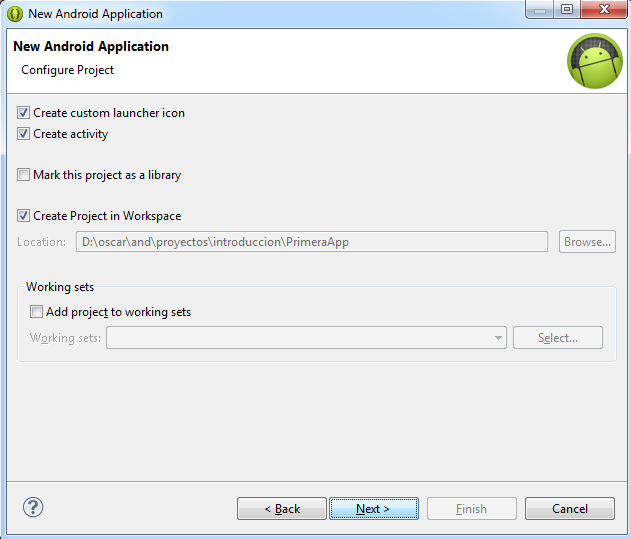
\includegraphics{asistente2.png}}
\caption{Opciones específicas del proyecto}{\small 
Aquí podremos indicar si queremos crear una biblioteca en lugar de una aplicación, si deseamos que se cree una actividad en blanco y si queremos ponerlo en el directorio de trabajo predeterminado. Se dejarán las opciones por defecto.
}\end{figure}
\begin{figure}[htbp]
\centering
\capstart

\scalebox{0.500000}{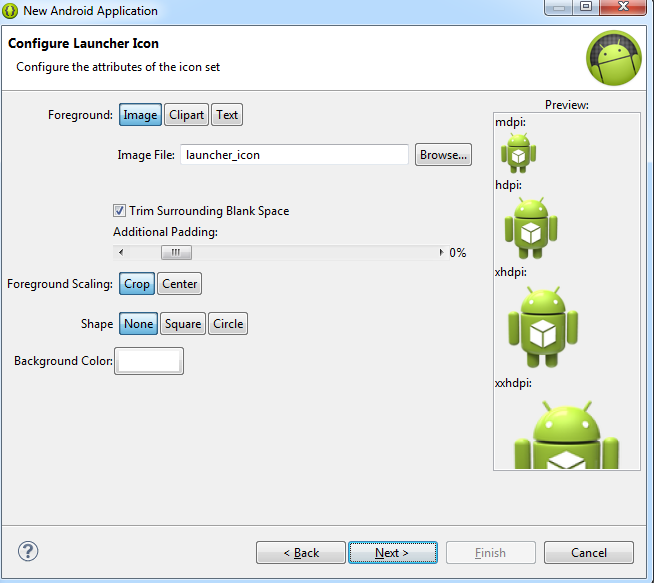
\includegraphics{asistente3.png}}
\caption{Personalizando el icono}{\small 
Esta ventana permite elegir algunas opciones sobre el icono de la aplicación:
}\end{figure}
\begin{figure}[htbp]
\centering
\capstart

\scalebox{0.500000}{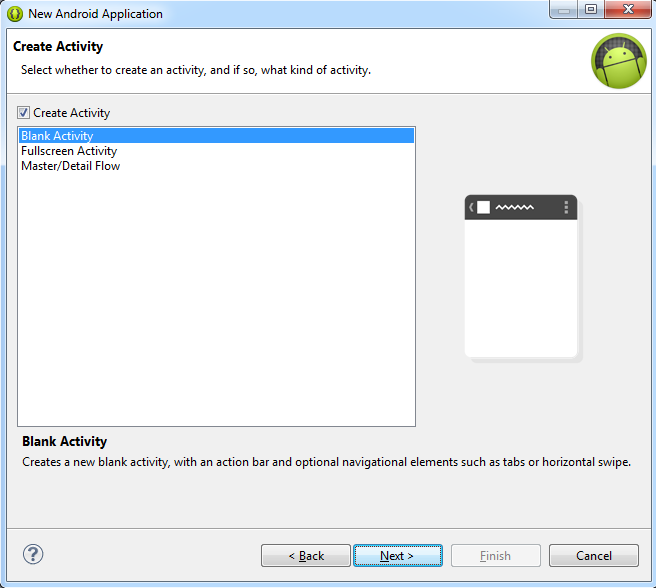
\includegraphics{asistente4.png}}
\caption{Tipo de actividad}{\small 
Aquí se puede elegir que tipo de actividad se desea. En general, usaremos una actividad en blanco.
}\end{figure}
\begin{figure}[htbp]
\centering
\capstart

\scalebox{0.500000}{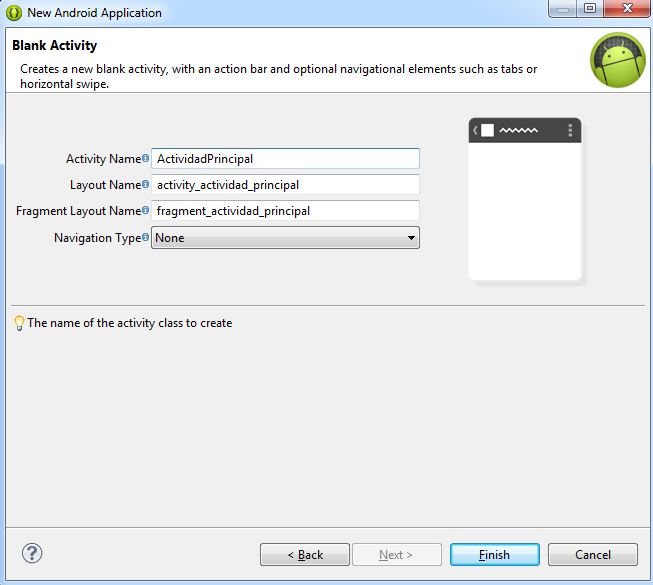
\includegraphics{asistente5.png}}
\caption{Datos de la actividad}{\small 
En este último paso se indicará el nombre de la clase que contendrá la actividad principal de la aplicación. Usaremos el nombre \code{ActividadPrincipal} y terminaremos el asistente.
}\end{figure}
\begin{figure}[htbp]
\centering
\capstart

\scalebox{0.500000}{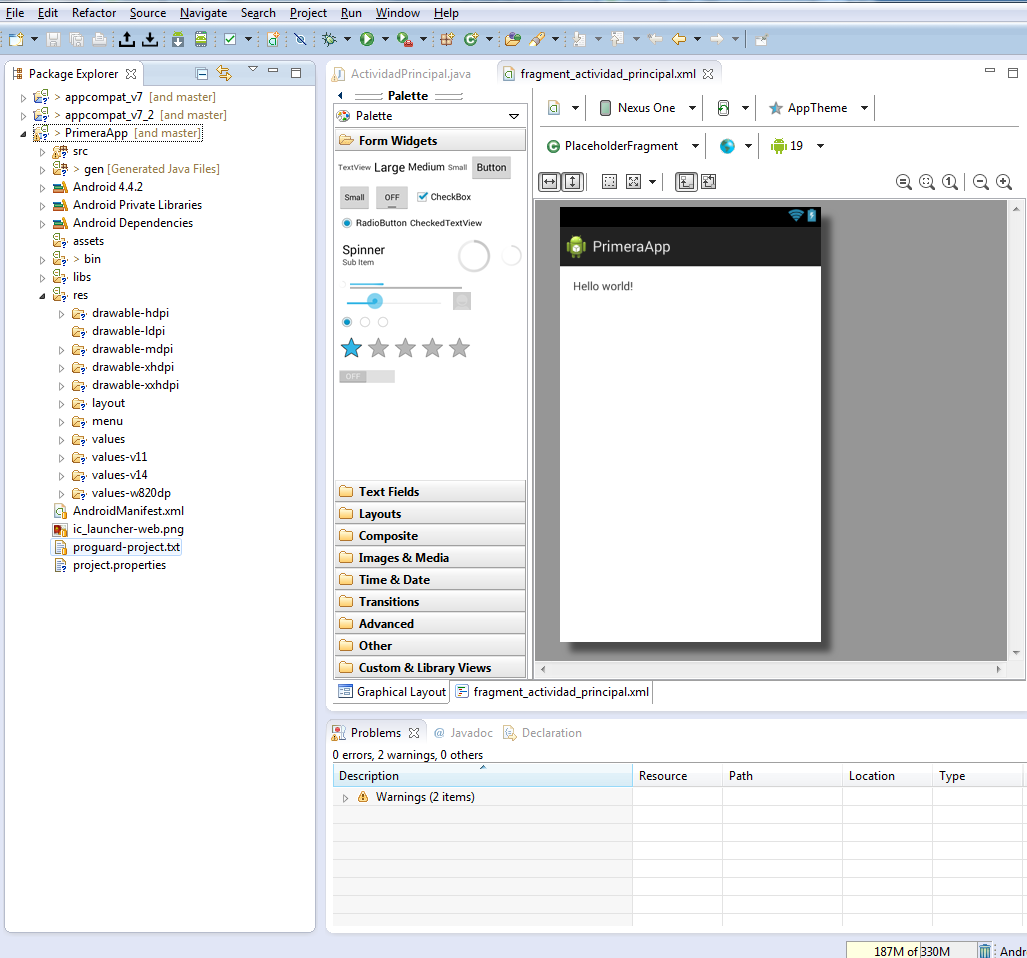
\includegraphics{proyectovacio.png}}
\caption{Un proyecto vacío de Android}{\small 
El asistente terminará y se nos mostrará el entorno de Eclipse.
}\end{figure}


\section{Descargando plataformas}
\label{index:descargando-plataformas}
Una vez hecho esto se debería instalar alguna versión del kit de desarrollo Android para empezar a programar. Para ello, se debe arrancar el gestor de plataformas Android mediante el menú de Eclipse \code{Window-\textgreater{}SDK Manager}
\begin{figure}[htbp]
\centering
\capstart

\scalebox{0.500000}{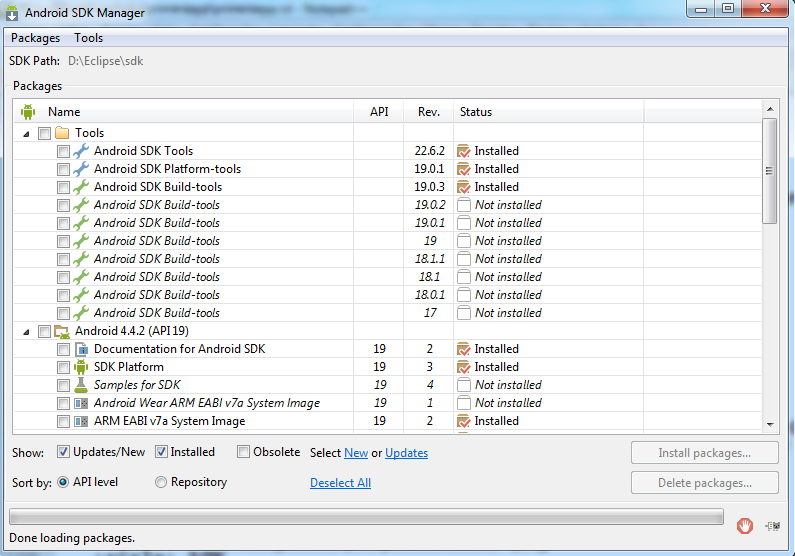
\includegraphics{sdkmanager.png}}
\caption{Administrador de plataformas Android}\end{figure}

El SDK Manager hace unas cuantas recomendaciones bastante prácticas: normalmente intentará instalar la última versión de Android más algunas herramientas útiles.

\begin{notice}{warning}{Advertencia:}
Una de las herramientas que se descargará es \emph{Intel x86 Emulator Accelerator} o HAXM. \href{http://software.intel.com/en-us/android/articles/intel-hardware-accelerated-execution-manager}{Esta herramienta de Intel} permite acelerar la ejecución del emulador de Android en microprocesadores Intel que tengan activada en su BIOS la opción de aceleración. Puede ser necesario habilitar esta opción en la BIOS (probablemente en alguna opción con el nombre \code{Enable Intel VT-x} o similar). El uso de HAXM es \textbf{MUY RECOMENDABLE}. Por otro lado, el SDK Manager descarga, pero no descomprime ni instala HAXM. Se debe buscar el ZIP en el directorio de instalación y ejecutarlo.
\end{notice}

En líneas generales se necesitarán:
\begin{itemize}
\item {} 
Todos los archivos de la última plataforma

\item {} 
El driver USB, que permitirá ejecutar nuestros programas en un móvil/tablet conectado por USB al equipo

\item {} 
El driver HAXM

\item {} 
La biblioteca de soporte de Android: permite que programas con una versión moderna se ejecuten en algunas plataformas más antiguas, entre otras cosas.

\item {} 
Las \emph{build-tools} o herramientas de compilación.

\item {} 
Las \emph{platform-tools} o herramientas específicas de la plataforma.

\item {} 
Las \emph{Android tools}, herramientas específicas de Android

\end{itemize}


\section{Creando emuladores}
\label{index:creando-emuladores}
Cuando se haya completado el paso anterior, se podrán crear \emph{Android Virtual Devices} o AVDs o emuladores. Se pueden crear dispositivos con diferentes características como se muestra a continuación.

En primer lugar, se debe elegir la opción \code{Window-Android Virtual Device Manager}, con lo que ser verá una herramienta que permite crear emuladores.
\begin{figure}[htbp]
\centering
\capstart

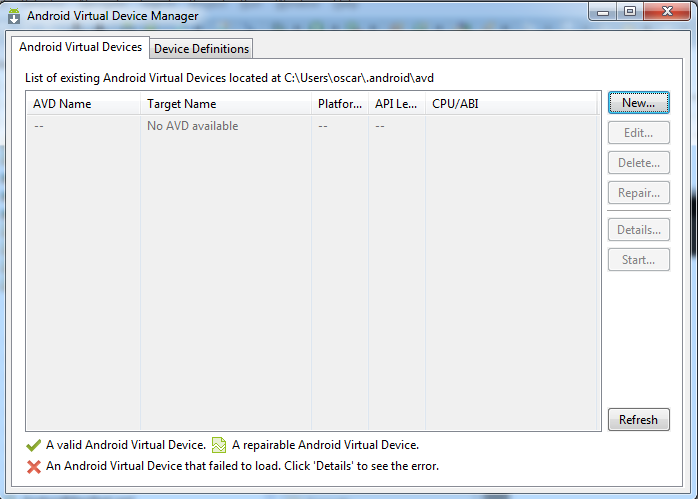
\includegraphics{avdmanager.png}
\caption{El Android Virtual Device Manager}\end{figure}
\begin{figure}[htbp]
\centering
\capstart

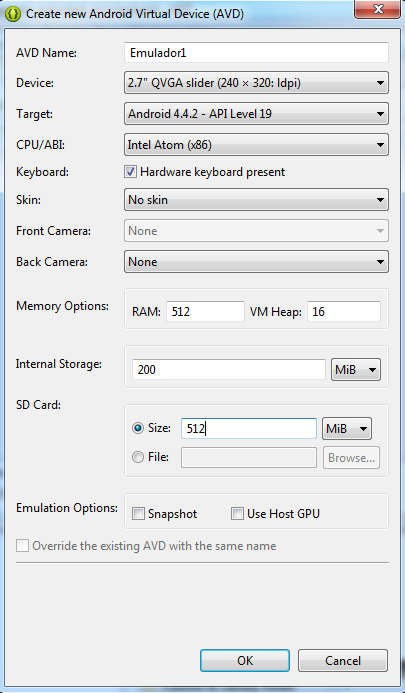
\includegraphics{creandoavd.png}
\caption{Creando dispositivos}{\small 
Una vez arrancado se podrá crear un nuevo dispositivo con el botón \emph{New}. Se recomienda mantener estas opciones.
}\end{figure}


\section{Arrancando el programa}
\label{index:arrancando-el-programa}
Una vez que se tiene el emulador creado, se puede arrancar con el botón Start, y despues arrancar el proyecto vacío Android de Eclipse. Para ello, una posibilidad es hacer click con el botón derecho en el proyecto que vemos a la izquierda de Eclipse y elegir el menu \code{Run As-Android Application}. Debería arrancarse la aplicación en el emulador y ver el resultado.
\begin{figure}[htbp]
\centering
\capstart

\scalebox{0.500000}{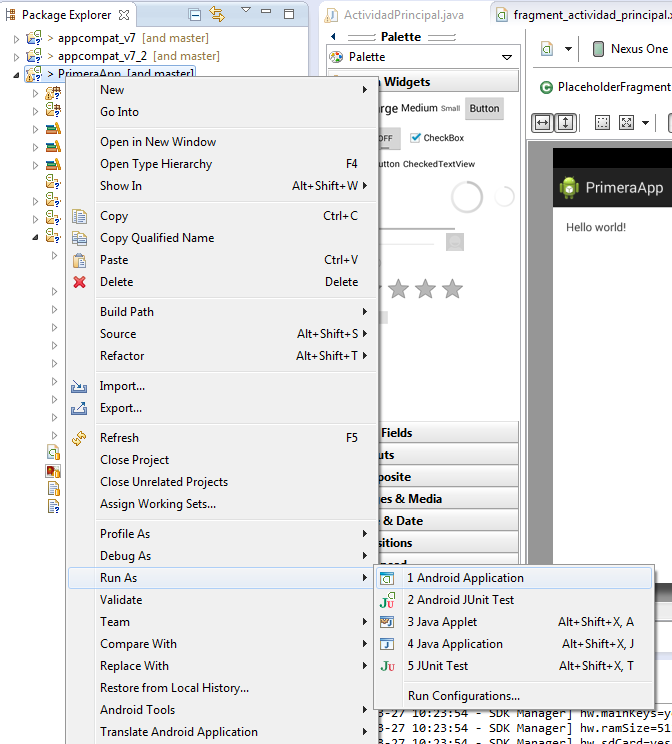
\includegraphics{ejecutandovacio.png}}
\caption{Ejecutando el primer proyecto}\end{figure}
\begin{figure}[htbp]
\centering
\capstart

\scalebox{0.500000}{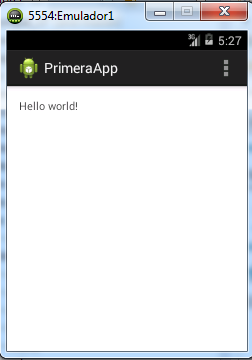
\includegraphics{primeraapp.png}}
\caption{Emulador ejecutando la primera app}\end{figure}


\section{Módulos para el desarrollo de aplicaciones móviles.}
\label{index:modulos-para-el-desarrollo-de-aplicaciones-moviles}
En este curso, realmente solo necesitaremos Java para crear apps. Sin embargo, existen un montón de bibliotecas que permiten acelerar el desarrollo.
\begin{itemize}
\item {} 
Unity para desarrollar juegos.

\item {} 
JQuery para Javascript.

\item {} 
Bibliotecas para tareas muy específicas como la seguridad SSL y similares.

\end{itemize}


\section{Emuladores.}
\label{index:emuladores}
A la hora de probar un app suele ser posible utilizar un emulador cargado en el sistema operativo que facilite la tarea de depurar la aplicación.

En Android, Google proporciona un sistema completo de emulación basado en máquinas virtuales (no usa VirtualBox sino un programa similar llamado QEMU).

El sistema de emulación permite crear dispositivos de características muy variadas para probar nuestra app en distintos entornos. Google denomina a estos dispositivos Android Virtual Devices (o AVDs)
\begin{itemize}
\item {} 
Se puede modificar el tamaño y la resolución.

\item {} 
La memoria RAM y espacio en tarjeta SD.

\item {} 
Se puede poner o quitar cámara.

\item {} 
Existen dispositivos predefinidos por Google que permiten crear emuladores muy rápidamente.

\item {} 
También se pueden clonar dispositivos para hacer solo una modificación de forma rápida.

\item {} 
Una característica de interés es que \emph{si se dispone de una tarjeta gráfica con aceleración} se puede activar una casilla llamada ``Host GPU'' que permite acelerar la emulación.

\item {} 
Se puede obligar al emulador a que ``recuerde'' el estado en que se quedó para así continuar donde nos hubiésemos quedado el último día. Esta opción se llama instantánea o \emph{snapshot}.

\end{itemize}

Si el equipo de escritorio es un Intel se puede instalar el Hardware Accelerated eXecution Manager o HAXM que permite acelerar la emulación. En el directorio \code{sdk/extras/intel} se puede encontrar un archivo ZIP que contiene un EXE que instala el HAXM. Se recomienda encarecidamente instalarlo en casa y, si es necesario, habilitar la tecnología VT en la BIOS.


\section{Ciclo de vida}
\label{index:ciclo-de-vida}\begin{figure}[htbp]
\centering
\capstart

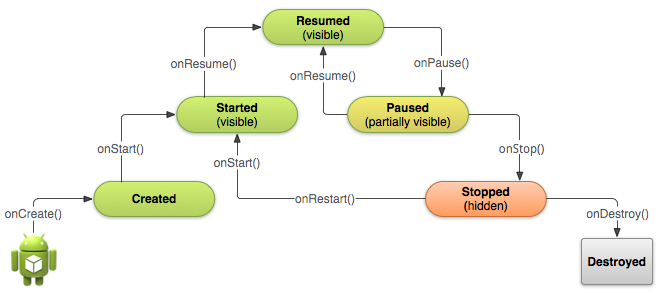
\includegraphics{ciclodevida.png}
\caption{Pasos en la ejecución de una app (imagen tomada de Google).}\end{figure}


\section{Configuraciones y perfiles}
\label{index:configuraciones-y-perfiles}

\section{Modificación de aplicaciones existentes.}
\label{index:modificacion-de-aplicaciones-existentes}

\section{Utilización del entorno de ejecución del administrador de aplicaciones.}
\label{index:utilizacion-del-entorno-de-ejecucion-del-administrador-de-aplicaciones}

\chapter{Programación de aplicaciones para dispositivos móviles}
\label{index:programacion-de-aplicaciones-para-dispositivos-moviles}

\section{Herramientas y fases de construcción.}
\label{index:herramientas-y-fases-de-construccion}

\section{Interfaces de usuario. Clases asociadas.}
\label{index:interfaces-de-usuario-clases-asociadas}

\section{Servicios en dispositivos móviles.}
\label{index:servicios-en-dispositivos-moviles}

\section{Proveedores de contenido.}
\label{index:proveedores-de-contenido}

\section{Gestión de recursos y notificaciones.}
\label{index:gestion-de-recursos-y-notificaciones}

\section{Contexto gráfico. Imágenes.}
\label{index:contexto-grafico-imagenes}

\section{Eventos del teclado.}
\label{index:eventos-del-teclado}

\section{Técnicas de animación y sonido.}
\label{index:tecnicas-de-animacion-y-sonido}

\section{Descubrimiento de servicios.}
\label{index:descubrimiento-de-servicios}

\section{Bases de datos y almacenamiento.}
\label{index:bases-de-datos-y-almacenamiento}

\section{Persistencia.}
\label{index:persistencia}

\section{Modelo de hilos.}
\label{index:modelo-de-hilos}

\section{Comunicaciones: clases asociadas. Tipos de conexiones.}
\label{index:comunicaciones-clases-asociadas-tipos-de-conexiones}

\section{Gestión de la comunicación inalámbrica.}
\label{index:gestion-de-la-comunicacion-inalambrica}

\section{Seguridad y permisos.}
\label{index:seguridad-y-permisos}

\section{Envío y recepción de mensajes texto.}
\label{index:envio-y-recepcion-de-mensajes-texto}

\section{Envío y recepción de mensajería multimedia. Sincronización de contenido.}
\label{index:envio-y-recepcion-de-mensajeria-multimedia-sincronizacion-de-contenido}

\section{Manejo de conexiones HTTP y HTTPS.}
\label{index:manejo-de-conexiones-http-y-https}

\section{Empaquetado y despliegue de aplicaciones para dispositivos móviles.}
\label{index:empaquetado-y-despliegue-de-aplicaciones-para-dispositivos-moviles}

\section{Centros de distribución de aplicaciones.}
\label{index:centros-de-distribucion-de-aplicaciones}

\section{Documentación de aplicaciones de dispositivos móviles.}
\label{index:documentacion-de-aplicaciones-de-dispositivos-moviles}

\chapter{Utilización de librerías multimedia integradas}
\label{index:utilizacion-de-librerias-multimedia-integradas}

\section{Conceptos sobre aplicaciones multimedia.}
\label{index:conceptos-sobre-aplicaciones-multimedia}

\section{Arquitectura del API utilizado.}
\label{index:arquitectura-del-api-utilizado}

\section{Fuentes de datos multimedia. Clases.}
\label{index:fuentes-de-datos-multimedia-clases}

\section{Datos basados en el tiempo.}
\label{index:datos-basados-en-el-tiempo}

\section{Procesamiento de objetos multimedia. Clases. Estados, métodos y eventos.}
\label{index:procesamiento-de-objetos-multimedia-clases-estados-metodos-y-eventos}

\section{Reproducción de objetos multimedia. Clases. Estados, métodos y eventos.}
\label{index:reproduccion-de-objetos-multimedia-clases-estados-metodos-y-eventos}

\section{Depuración y documentación de los programas.}
\label{index:depuracion-y-documentacion-de-los-programas}

\chapter{Análisis de motores de juegos}
\label{index:analisis-de-motores-de-juegos}

\section{Animación 2D y 3D.}
\label{index:animacion-2d-y-3d}

\section{Arquitectura del juego. Componentes.}
\label{index:arquitectura-del-juego-componentes}

\section{Motores de juegos: Tipos y utilización.}
\label{index:motores-de-juegos-tipos-y-utilizacion}

\section{Áreas de especialización, librerías utilizadas y lenguajes de programación}
\label{index:areas-de-especializacion-librerias-utilizadas-y-lenguajes-de-programacion}

\section{Componentes de un motor de juegos.}
\label{index:componentes-de-un-motor-de-juegos}

\section{Librerías que proporcionan las funciones básicas de un Motor 2D/3D.}
\label{index:librerias-que-proporcionan-las-funciones-basicas-de-un-motor-2d-3d}

\section{APIs gráficos 3D.}
\label{index:apis-graficos-3d}

\section{Estudio de juegos existentes.}
\label{index:estudio-de-juegos-existentes}

\section{Aplicación de modificaciones sobre juegos existentes.}
\label{index:aplicacion-de-modificaciones-sobre-juegos-existentes}

\chapter{Desarrollo de juegos 2D y 3D}
\label{index:desarrollo-de-juegos-2d-y-3d}

\section{Entornos de desarrollo para juegos.}
\label{index:entornos-de-desarrollo-para-juegos}

\section{Integración del motor de juegos en entornos de desarrollo.}
\label{index:integracion-del-motor-de-juegos-en-entornos-de-desarrollo}

\section{Conceptos avanzados de programación 3D.}
\label{index:conceptos-avanzados-de-programacion-3d}

\section{Fases de desarrollo:}
\label{index:fases-de-desarrollo}

\section{Propiedades de los objetos: luz, texturas, reflejos, sombras.}
\label{index:propiedades-de-los-objetos-luz-texturas-reflejos-sombras}

\section{Aplicación de las funciones del motor gráfico. Renderización.}
\label{index:aplicacion-de-las-funciones-del-motor-grafico-renderizacion}

\section{Aplicación de las funciones del grafo de escena.}
\label{index:aplicacion-de-las-funciones-del-grafo-de-escena}

\section{Tipos de nodos y su utilización.}
\label{index:tipos-de-nodos-y-su-utilizacion}

\section{Asociación de sonidos a los eventos del juego.}
\label{index:asociacion-de-sonidos-a-los-eventos-del-juego}

\section{Análisis de ejecución. Optimización del código.}
\label{index:analisis-de-ejecucion-optimizacion-del-codigo}

\section{Documentación de la fase de diseño y de desarrollo.}
\label{index:documentacion-de-la-fase-de-diseno-y-de-desarrollo}

\chapter{Sistemas basados en localización}
\label{index:sistemas-basados-en-localizacion}

\section{Tecnologías de localización (GPS, A-GPS,...).}
\label{index:tecnologias-de-localizacion-gps-a-gps}

\section{Servicios de localización, mapas y geocodificación.}
\label{index:servicios-de-localizacion-mapas-y-geocodificacion}

\section{Emuladores para simular las ubicaciones.}
\label{index:emuladores-para-simular-las-ubicaciones}

\section{Visualización la información geolocalizada.}
\label{index:visualizacion-la-informacion-geolocalizada}


\renewcommand{\indexname}{Índice}
\printindex
\end{document}
